\begin{figure}[t]
 \centering
 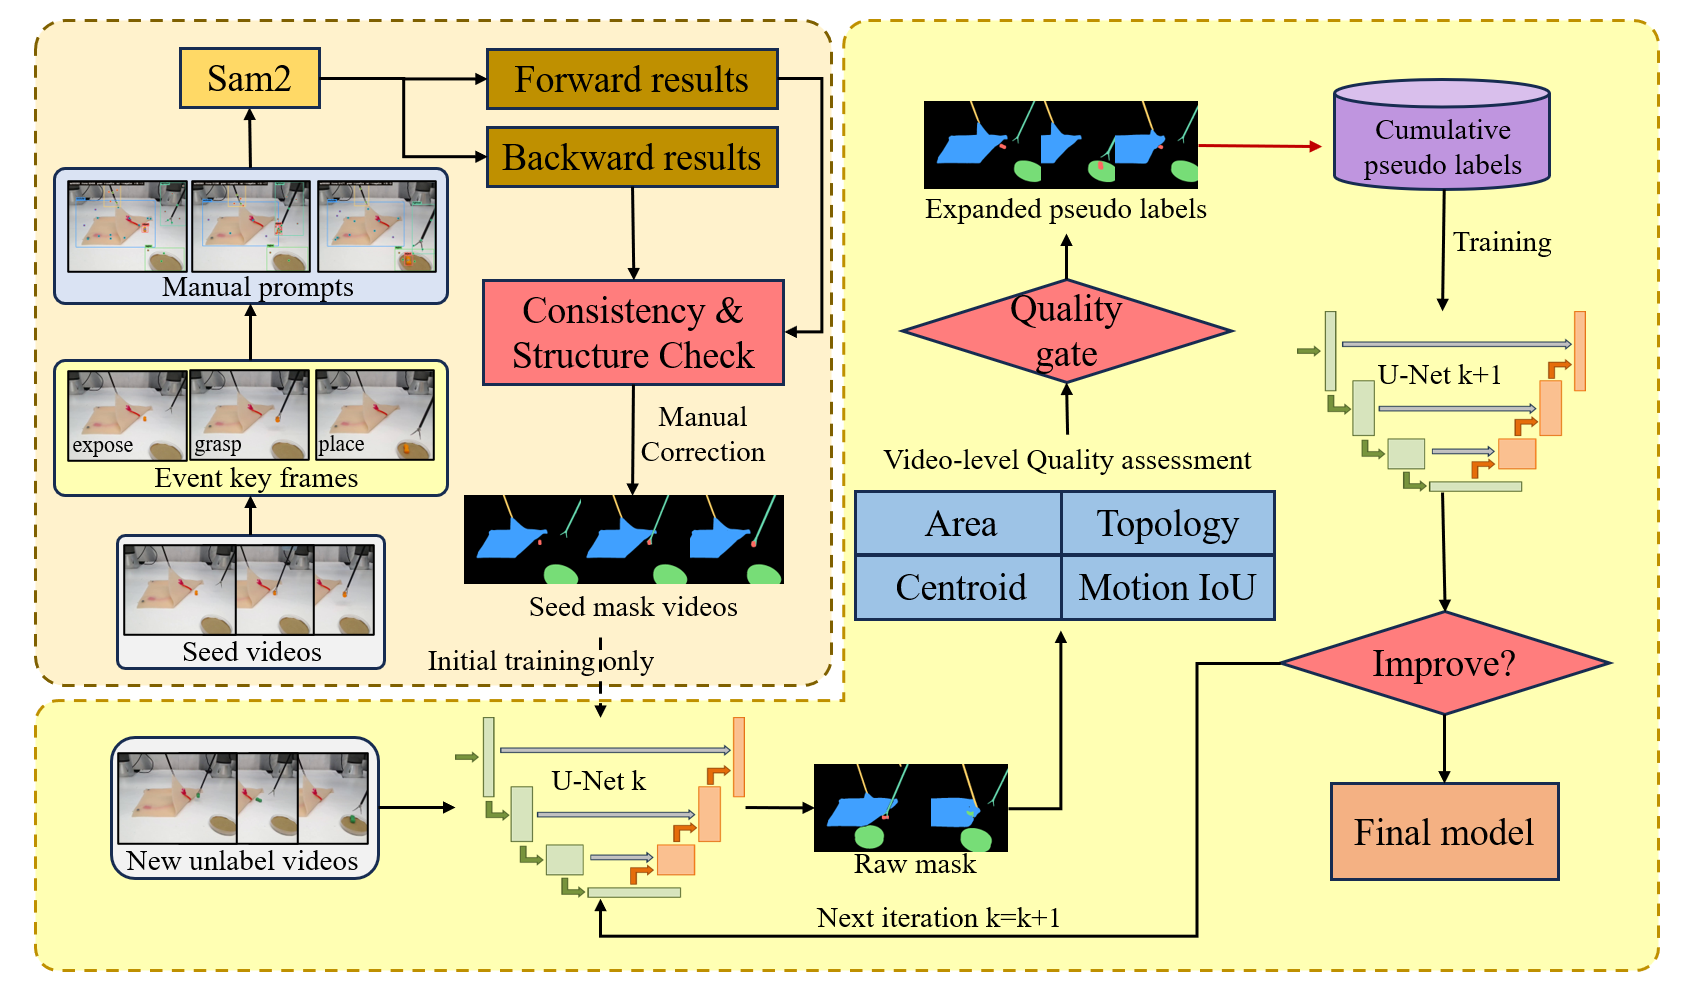
\includegraphics[width=\columnwidth]{myfigure/image3.png}
 % 审核后得到种子；后续仅使用累积的合格伪标签训练。
 \caption{Quality-aware iterative annotation. Reviewed bidirectional SAM2 masks train the initial segmenter. Subsequent models learn from cumulative, quality-screened pseudo-labels; seed videos are retained for reference rather than further training.}
 \label{fig:iterative-semantic-annotation}
\end{figure}
\section{Method}
\label{sec:method}
Section~\ref{sec:analysis} motivates preserving information relevant to expert action selection.
Figure~\ref{fig:architecture} organizes this approach into two components.
% 离线质量筛选迭代扩展少量人工审核标注。
First, quality-aware iterative annotation expands a small manually reviewed seed set into semantic supervision.
% RGB、语义和受监督查询共同支持基础动作块预测。
Second, RGB observations, semantic maps, and supervised task-descriptor queries jointly support a base action-chunk policy.

\subsection{Quality-Aware Iterative Semantic Supervision}
\label{sec:methodseg}
% 语义掩码决定描述量标签的质量，因而需控制错误伪标签在迭代中的传播。
Task-descriptor labels are derived from semantic masks, so segmentation errors can compromise the supervision used to preserve task information.
% 从少量审核种子出发，视频级筛选控制扩展标注的可靠性。
We combine reviewed seed annotations with video-level quality screening to limit error propagation as the labeled set expands (Fig.~\ref{fig:iterative-semantic-annotation}).

\subsubsection{Event-Guided Seeds and Iterative Expansion}
% 从覆盖主要交互与遮挡变化的少量视频中选择关键帧。
We select a small set of videos spanning the principal interaction and occlusion states, and annotate keyframes around events such as target exposure, contact, and placement.
% 人工框与正负点经SAM2双向传播，检查分歧并人工修正后得到种子掩码。
Bounding boxes and positive and negative point prompts guide bidirectional SAM2 propagation~\cite{ravi2024sam2}; consistency checks, class-dependent structural processing, and manual correction produce the seed masks.
% 种子训练初始U-Net，后续在新视频上生成候选标注。
The seeds train an initial U-Net segmenter, which predicts candidate masks on new unlabeled videos.
% 质量合格的标注跨轮累积，每轮重新初始化训练，种子不再用于后续拟合。
Accepted masks accumulate across iterations, and each subsequent segmenter is reinitialized and trained on this cumulative pool without the original seed videos.
% 种子改为固定参考，依据分割精度和异常率监测迭代。
The seed videos then serve as a fixed reference for monitoring segmentation accuracy and temporal anomalies.
% 不固定迭代次数，以精度保持条件下的异常改善作为继续依据。
Iteration continues while anomaly rates improve without a material loss of segmentation accuracy.

\subsubsection{Video-Level Quality Screening}
% 质量评估需要区分真实任务变化与偶发分割异常。
The screening procedure distinguishes sustained task changes from transient segmentation anomalies.
% 按类别从完整视频提取规模、空间位置与拓扑轨迹，并进行分段鲁棒建模。
For each class, we extract trajectories of mask area, spatial extent, centroid, and topology, and fit robust piecewise trends over the video.
% 持续变化允许新的状态段，短时偏离作为异常证据，而不是直接惩罚帧间差异。
Persistent changes can establish new segments, while short-lived departures provide anomaly evidence instead of penalizing every inter-frame change.
% 通过可靠光流对应计算运动补偿后的掩码IoU。
Motion-compensated mask IoU supplies additional temporal evidence on pixels with forward--backward-consistent optical-flow correspondences.
% 四类证据分别反映规模、空间形状、拓扑与运动不一致。
For class $c$ at frame $t$, we collect these diagnostics as
\begin{equation}
 \bm\upsilon_{t,c}^{\mathrm{seg}}
 =(\upsilon_{t,c}^{\mathrm{area}},
   \upsilon_{t,c}^{\mathrm{space}},
   \upsilon_{t,c}^{\mathrm{topo}},
   \upsilon_{t,c}^{\mathrm{motion}}).
 \label{eq:segevidence}
\end{equation}
% 多类证据共同识别异常，避免由单一面积或运动变化决定标签无效。
Agreement across evidence groups identifies anomalous intervals; excessive changes introduced by structural processing also trigger exclusion.
% 帧内相关类别均通过检查时才进入后续分割训练。
A frame enters subsequent segmentation training only when its relevant classes pass these checks.
% 人工参考用于发现时间上稳定的系统性误分。
The manually reviewed reference set complements temporal screening by checking for persistent semantic errors that temporal consistency alone cannot detect.
% 分割准入与描述量权重共享诊断来源，但依照各自监督对象使用。
The same diagnostics also determine descriptor-specific supervision weights in Section~\ref{sec:methodrelations}.
% 离线质量建模与在线分割明确分开，在线仅需当前图像。
Quality assessment is performed offline; the final per-view segmenters are frozen and require only current images during policy execution.

\subsection{Semantic Inputs and Task-Descriptor Queries}
\label{sec:methodrelations}
% 语义突出对象级结构，查询监督引导表示保留具体任务信息。
Semantic maps emphasize object-level spatial structure, while supervised queries encourage the joint representation to retain task-relevant attributes and relationships.
% RGB与本体信息保留类别图无法完整表达的决策线索。
RGB and proprioception remain available for decision cues not captured by the semantic classes.
% 这对应C中的描述量估计途径，而非声称增加输入自动改善覆盖。
This design targets the descriptor-estimation term in~\eqref{eq:expertreconstruction} through the learned representation, rather than assuming that adding semantic channels improves coverage.

\subsubsection{Joint Visual-Semantic Encoding}
% 冻结的各视角分割器输出类别概率，并以固定颜色形成软语义图。
For view $v$, a frozen segmenter predicts class probabilities $p_t^v(c,\xi)$ from image $I_t^v$.
We form a soft semantic image as
\begin{equation}
 S_t^v(\xi)=\sum_{c\in\mathcal C_v}p_t^v(c,\xi)e_c^{\mathrm{sem}},
 \label{eq:methodsoftsem}
\end{equation}
% 定义类别集合、像素和固定颜色；不进行argmax硬化。
where $\mathcal C_v$ is the view-specific class set, $\xi$ a pixel location, and $e_c^{\mathrm{sem}}\in[0,1]^3$ a fixed class color.
% 概率加权颜色图允许共享三通道编码器。
This probability-weighted color representation allows RGB and semantics to use the same three-channel visual encoder without argmax hardening.
% 各输入流分别编码后与本体信息和查询进入Transformer。
The encoded streams from all views are combined with proprioceptive and query tokens in a transformer encoder.
% ACT作为基础实例，不展开其标准生成结构。
An ACT decoder~\cite{zhao2023act} reads this context to predict the base action chunk.

\subsubsection{Supervised Descriptor Queries}
% 按任务选择描述量组，组成理论中的向量G。
We select $K_{\mathrm{rel}}$ descriptor groups $G^{(j)}\in\R^{d_j}$, such as visible area and relative position, which together form the task descriptor vector $G$.
% 标签来自离线语义掩码，具体任务定义放在附录。
Fixed geometric operators applied to the offline masks generate pseudo-labels $\widetilde G_t^{(j)}$; the task-specific definitions are given in Appendix~\ref{app:descriptorinstance}.
% 每组一个查询，查询输出同时用于辅助读出与动作解码。
Each group has a learnable query whose encoded output $z_t^{(j)}$ supports a prediction head,
$\widehat G_t^{(j)}=D_j(z_t^{(j)})$, and remains available to the action decoder.
% 约束的是可读出的任务信息，不是指定注意力图。
Supervision therefore encourages task information to be recoverable from the policy representation without prescribing an attention map.

% 描述量权重依据自身有效性与相关类别的质量，避免无关异常影响监督。
A weight $\varpi_{n,j}^{G}\in[0,1]$ combines descriptor validity with quality evidence from the relevant semantic classes.
% 可信、存疑及异常标签分别全量、降权或停用。
Reliable labels receive full weight, uncertain labels are downweighted, and undefined or anomalous labels receive zero weight.
% 无定义距离与确认的零面积需要区分。
In particular, a distance is undefined when either object is invisible, whereas a confirmed absence can provide a valid zero-visible-area label.
% 只停止辅助监督，不删除动作示范。
Disabling a descriptor loss does not remove the sample's action supervision.
% 将组内尺度归一化后的向量误差写为紧凑的辅助损失。
With descriptors normalized to fixed scales, the training objective is
\begin{align}
 \mathcal L_{\mathrm{rel}}
 &=\frac{1}{K_{\mathrm{rel}}}\sum_j
   \frac{\sum_n\varpi_{n,j}^{G}
      \ell_G(\widehat G_n^{(j)}-\widetilde G_n^{(j)})}
        {\max(1,\sum_n\varpi_{n,j}^{G})},\nonumber\\
 \mathcal L_{\mathrm{base}}
 &=\mathcal L_{\mathrm{IL}}
   +\lambda_{\mathrm{rel}}\mathcal L_{\mathrm{rel}}.
 \label{eq:methodbaseloss}
\end{align}
% 定义批索引、分量平均损失和ACT原有训练目标。
Here, $n$ indexes minibatch samples, $\ell_G$ is the component-averaged Smooth L1 loss, and $\mathcal L_{\mathrm{IL}}$ is the standard ACT training objective.
% 质量权重仅用于监督，分割器始终冻结。
The segmenters remain frozen, and quality weights affect auxiliary supervision rather than online policy inputs.
% 附录仅补充标签准入及其与描述量误差的关系。
Appendices~\ref{app:seguncertainty} and~\ref{app:pseudolabel} specify label admission and its connection to descriptor-estimation error.

